% vim: nu expandtab shiftwidth=2 softtabstop=2 foldmethod=marker
\section{Homework 5}

\lstset{language=C++,
	frame=tb,
	tabsize=2,
	showstringspaces=false,
	commentstyle=\color{green},
	keywordstyle=\color{blue},
	stringstyle =\color{red}}

Upon completing this assignment, you will be able to empirically and theoretically analyze sorting algorithms

\begin{enumerate}
\item \textbf{Programming:} You are given C++ code for quicksort and another (very bad) sorting algorithm, called \textbf{badsort}. Modify the given code, so that
  \begin{enumerate}
  \item It will count the number of comparisons between objects in the input array for each sorting algorithm.
  \item It will calculate the \emph{real execution time} of each sorting algorithm.
  \item [] (Hint: use the function call \textbf{time(0)} to record the current time. Function \textbf{time()} is defined in the \textbf{ctime} library.)
  \item It allows the user to enter the length of an input array to be sorted, and choose either to enter values or to generate random numbers for the array elements. It also allows the user to view the randomly generated array if he/she wants to. Make sure that it will generate different sequences of random numbers at different runs of the program.
  \item It will call the two sorting algorithms on the same input array obtained from step (c) above, and display both the number of object comparisons and the real execution time for each sorting algorithm call. It also allows the user to view the output array for each sorting algorithm call if he/she wants to.
  \end{enumerate}
\item \textbf{Empirical Analysis:}
  \begin{enumerate}
  \item Run your program to sort an input array of \emph{n} random integers for \textbf{10} different values of \emph{n} in the range [10, 100]. Then report the number of comparisons of each sorting algorithm call in a table of the same format as Table 1 below.
\begin{table}
  \begin{center}
    \begin{tabular}{| c | c | c | c | c|}\hline
    \multicolumn{5}{|c|}{Number of Object Comparisons} \\ \hline
    n & quicksort & badsort & $n^{2}$ & $n\log{(n)}$ \\ \hline
  10  & 55        & 102     & 100     &  $33.2193$   \\ \hline
  20  & 134       & 890     & 400     &  $86.4386$   \\ \hline
  30  & 243       & 2799    & 900     & $147.2067$   \\ \hline
  40  & 307       & 7480    & 1600    & $212.8771$   \\ \hline
  50  & 436       & 13321   & 2500    & $282.1928$   \\ \hline
  60  & 579       & 20557   & 3600    & $354.4134$   \\ \hline
  70  & 632       & 34266   & 4900    & $429.0498$   \\ \hline
  80  & 750       & 60294   & 6400    & $505.7545$   \\ \hline
  90  & 902       & 81034   & 8100    & $584.2668$   \\ \hline
  100 & 1015      & 111456  & 10000   & $644.3856$   \\ \hline
    \end{tabular}\\
  \caption{Number of Object Comparisons}
  \label{tab:numberofobjectcomparisons}
  \end{center}
\end{table}
  \item Run your program to sort an input array of \emph{n} random integers for \textbf{5} different values of in the range [10000, 100000]. These runs must be done on the same computer. Then report the real execution time of each sorting algorithm call in a table of the same format as Table 2 below.
\begin{table}
  \begin{center}
    \begin{tabular}{|l | l | l|}\hline
    \multicolumn{3}{|c|}{Real Execution Time} \\ \hline
    n    & quicksort(ms) & badsort   \\ \hline
  10000  & $15.3238$     & $5416.88$ seconds \\ \hline
  11000  & $11.068$      & $7285.02$ seconds \\ \hline
  15000  & $16.9995$     & $18587.8$ seconds \\ \hline
  75000  & $127.086$     & $>5.67$ days   \\ \hline
 100000  &               & $>5.67$ days   \\ \hline
    \end{tabular}
  \caption{Real Execution Time}
  \label{tab:realexecutiontime}
  \end{center}
\end{table}
  \item Draw a line graph (using Excel) that shows the number of comparisons of each sorting algorithm call from your experiments in part (2a) as well as the two functions $n^{2}$ and $\log{(n)}$. So, there will be four lines in this graph.
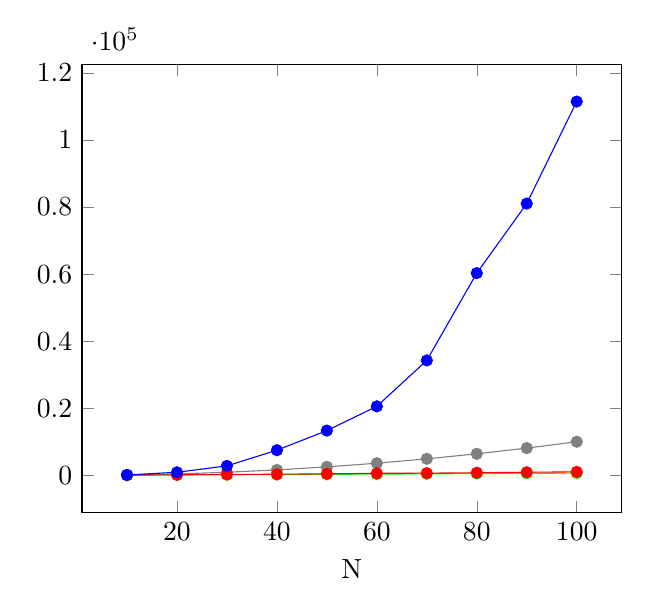
\begin{tikzpicture}
\begin{axis}[xlabel=N]
\addplot [color=gray, mark=*] coordinates{ %squared
  (10,  100)
  (20,  400)
  (30,  900)
  (40,  1600)
  (50,  2500)
  (60,  3600)
  (70,  4900)
  (80,  6400)
  (90,  8100)
  (100, 10000)};
\addplot [color=green, mark=*] coordinates{ %log(n)
  (10,  33.2193)
  (20,  86.4386)
  (30,  147.2067)
  (40,  212.8771)
  (50,  282.1928)
  (60,  354.4134)
  (70,  429.0498)
  (80,  505.7545)
  (90,  584.2668)
  (100, 644.3856)};
\addplot [color=red, mark=*] coordinates{ %quicksort
  (10,  55)
  (20,  134)
  (30,  243)
  (40,  307)
  (50,  436)
  (60,  579)
  (70,  632)
  (80,  750)
  (90,  902)
  (100, 1015)};
\addplot [color=blue, mark=*] coordinates{ %badsort
  (10,  102)
  (20,  890)
  (30,  2799)
  (40,  7480)
  (50,  13321)
  (60,  20557)
  (70,  34266)
  (80,  60294)
  (90,  81034)
  (100, 111456)};
\iffalse
\addplot [color=purple, samples=100, domain=0:10] coordinates{ %cubic
  (10, 1000)
  (20, 8000)
  (30, 27000)
  (40, 64000)
  (50, 125000)
  (60, 216000)
  (70, 343000)
  (80, 512000)
  (90, 729000)
  (100, 1000000)};
\addplot [color=purple, samples=100, domain=0:10] coordinates{ %n^5/2
(10, 316.227766017)
(20, 1788.854382)
(30, 4929.50301755)
(40, 10119.2885125)
(50, 17677.6695297)
(60, 27885.4800927)
(70, 40996.3413002)
(80, 57243.340224)
(90, 76843.3471421)
(100, 100000.0)};
\fi
\end{axis}
\end{tikzpicture}
  \item Draw a conclusion regarding the number of comparisons based on the graph, and draw another conclusion regarding the real execution time from your data collected in part 2b. 
    \begin{itemize}
    \item Looking at the graph of the number of comparisons, I believe badsort to be $\Theta(n^{3})$. If you add in the $n^{3}$ graph (green) and the graph of $n^{5/2}$(red), it closely matches the graph of $n^{5/2}$, but is just a little bit faster growing. From the original graph, it is clear that quicksort is $\Theta(\log{(n)})$ as the lines match fairly perfectly.
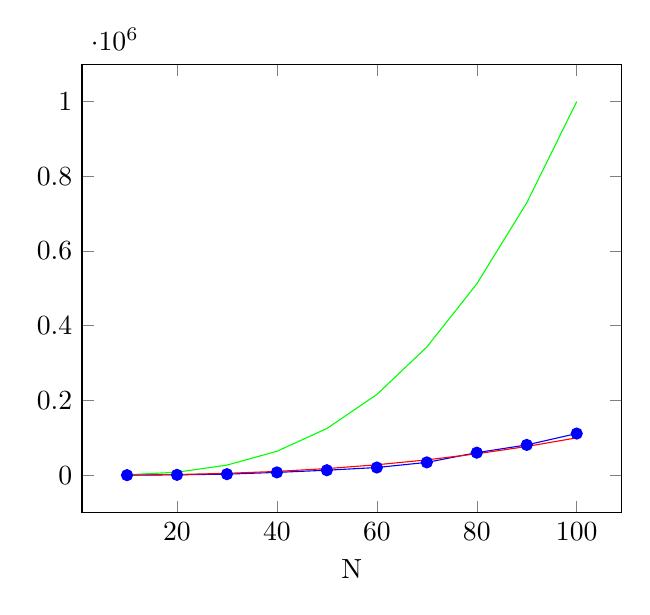
\begin{tikzpicture}
\begin{axis}[xlabel=N]
\addplot [color=blue, mark=*] coordinates{ %badsort
  (10,  102)
  (20,  890)
  (30,  2799)
  (40,  7480)
  (50,  13321)
  (60,  20557)
  (70,  34266)
  (80,  60294)
  (90,  81034)
  (100, 111456)};
\addplot [color=green, samples=100, domain=0:10] coordinates{ %cubic
  (10, 1000)
  (20, 8000)
  (30, 27000)
  (40, 64000)
  (50, 125000)
  (60, 216000)
  (70, 343000)
  (80, 512000)
  (90, 729000)
  (100, 1000000)};
\addplot [color=red, samples=100, domain=0:10] coordinates{ %n^5/2
(10, 316.227766017)
(20, 1788.854382)
(30, 4929.50301755)
(40, 10119.2885125)
(50, 17677.6695297)
(60, 27885.4800927)
(70, 40996.3413002)
(80, 57243.340224)
(90, 76843.3471421)
(100, 100000.0)};
\end{axis}
\end{tikzpicture}
    \item In order to draw a conclusion, we need to look at the economics of the modern computer, the modern supercomputer that is. There exists a single government computer that is powered by two full nuclear power plants, and syphons power from a third coal based power plant. This computer is somewhat open to scientists, and thus this code could possibly be run there if we assume it scales with MPI, which it does if we break our arrays into subsections and then are running bad sort or quicksort on each subarray, which is the normal programming practice. I know that the government computer draws five kilwatts of power while in use and that the wait queue times are directly proportional to the amount of time you want to run. For instance, in order to run for 24 hours on a smaller less used computer, the wait time is about 1 month. So lets assume that running your code uses the full power of the computer, and that each subarray is comparable to what was run, and that performance on each subarray is comparable and requires no extra setup time. In order to run quicksort, you would spend roughly 4 seconds in the queue and your program would run on roughly 0.17651 watts. Badsort on the other hand, would wait in the queue a minimum of 5.67 months in the queue, and use 680.4 kilowatts. We would use all of that, and still not be done sorting our array. I believe from this, its rather obvious to never use the badsort, as most people dont want to spend six months of their lives waiting for something that could take less than five seconds, but if you want to waste 6 months a few thousand watts of electricity, I guess thats up to you.
    \end{itemize}
  \end{enumerate}
\item \textbf{Theoretical Analysis:}
  \begin{enumerate}
  \item Analyze the space complexity for the \textbf{badsort} algorithm.
    \begin{itemize}
    \item The space complexity of the badsort algorithm is $\Theta(1)$. This is due to the algorithm only needing to store the array of n items a constant number of times (zero due to it being passed by reference), and there being nothing else tied to n, such as stack frames if this was a recursive function. You might think that because this function calls swap, and that because swapValues allocates new memory each time it is called, that this should play into the calculations. It does not because although swapValues is in the file, badsort actually calls the standard template library swap function, which does not allocate new memory and operates in constant time.
    \end{itemize}
  \item Analyze the worst-case time complexity for the \textbf{badsort} algorithm. For this part, you will have to \emph{estimate} the total number of object comparisons made by badsort:
    \begin{enumerate}
    \item Try to find a good aymptotic upper bound on the total number of object comparisons made by badsort on an input array of length \emph{n}
      \begin{itemize}
      \item In the worst case, the array is reverse sorted, the outer loop executed n! times.
      \item Using stirlings approximation from earlier in the course, we get $\sqrt{2\pi}n^{n+1/2}e^{-n}$
      \item So the asymtotic upper bound for the worst case is $O=n^{n+1/2}$
      \item In the best case, where the array is sorted, the upper bound is $O(n)$ as it just compares each thing and moves on.
      \item In the average case, we found from our graph that a good upperbound is $O(n^{3})$
      \item As the problem merely asks for an asymptotic upperbound, we must assume the worst case, $O=n^{n+1/2}$
      \end{itemize}
    \item Try to find a good asymptotic lower bound on the total number of object comparisons made by badsort on an input array of length \emph{n} in the \emph{reverse order}.
      \begin{itemize}
      \item Assuming reverse order means sorted from highest to lowest, or reverse sorted, then the asymptotic lower bound is $o=n^{n+1/2}$
      \end{itemize}
    \end{enumerate}
  \end{enumerate}
\end{enumerate}

\subsection{Given C++ code}
\lstinputlisting{Homework/Homework-5/C455-Sp16-Hw5-GivenCode.cpp}
\subsection{My C++ code}
\lstset{language=C++,
	frame=tb,
	showstringspaces=false,
	commentstyle=\color{green},
	keywordstyle=\color{blue},
	stringstyle =\color{red}}
\lstinputlisting{Homework/Homework-5/main.cpp}
\subsection{Makefile}
\lstset{basicstyle=\ttfamily,
        language=bash,
	frame=tb,
	showstringspaces=false,
	commentstyle=\color{green},
	keywordstyle=\color{blue},
	stringstyle =\color{red}}
\lstinputlisting{Homework/Homework-5/Makefile}
